\chapter{Modeller} \label{chap:klasser}

I dette kapitel vil klasserne i modellaget blive beskrevet.
Den overordnede klassestruktur er beskrevet i UML--diagrammet på \myref{img:UML}, heri kan alle de konkrete felter som findes i hver klasse ses.

\begin{figure}[H]
  \centering
  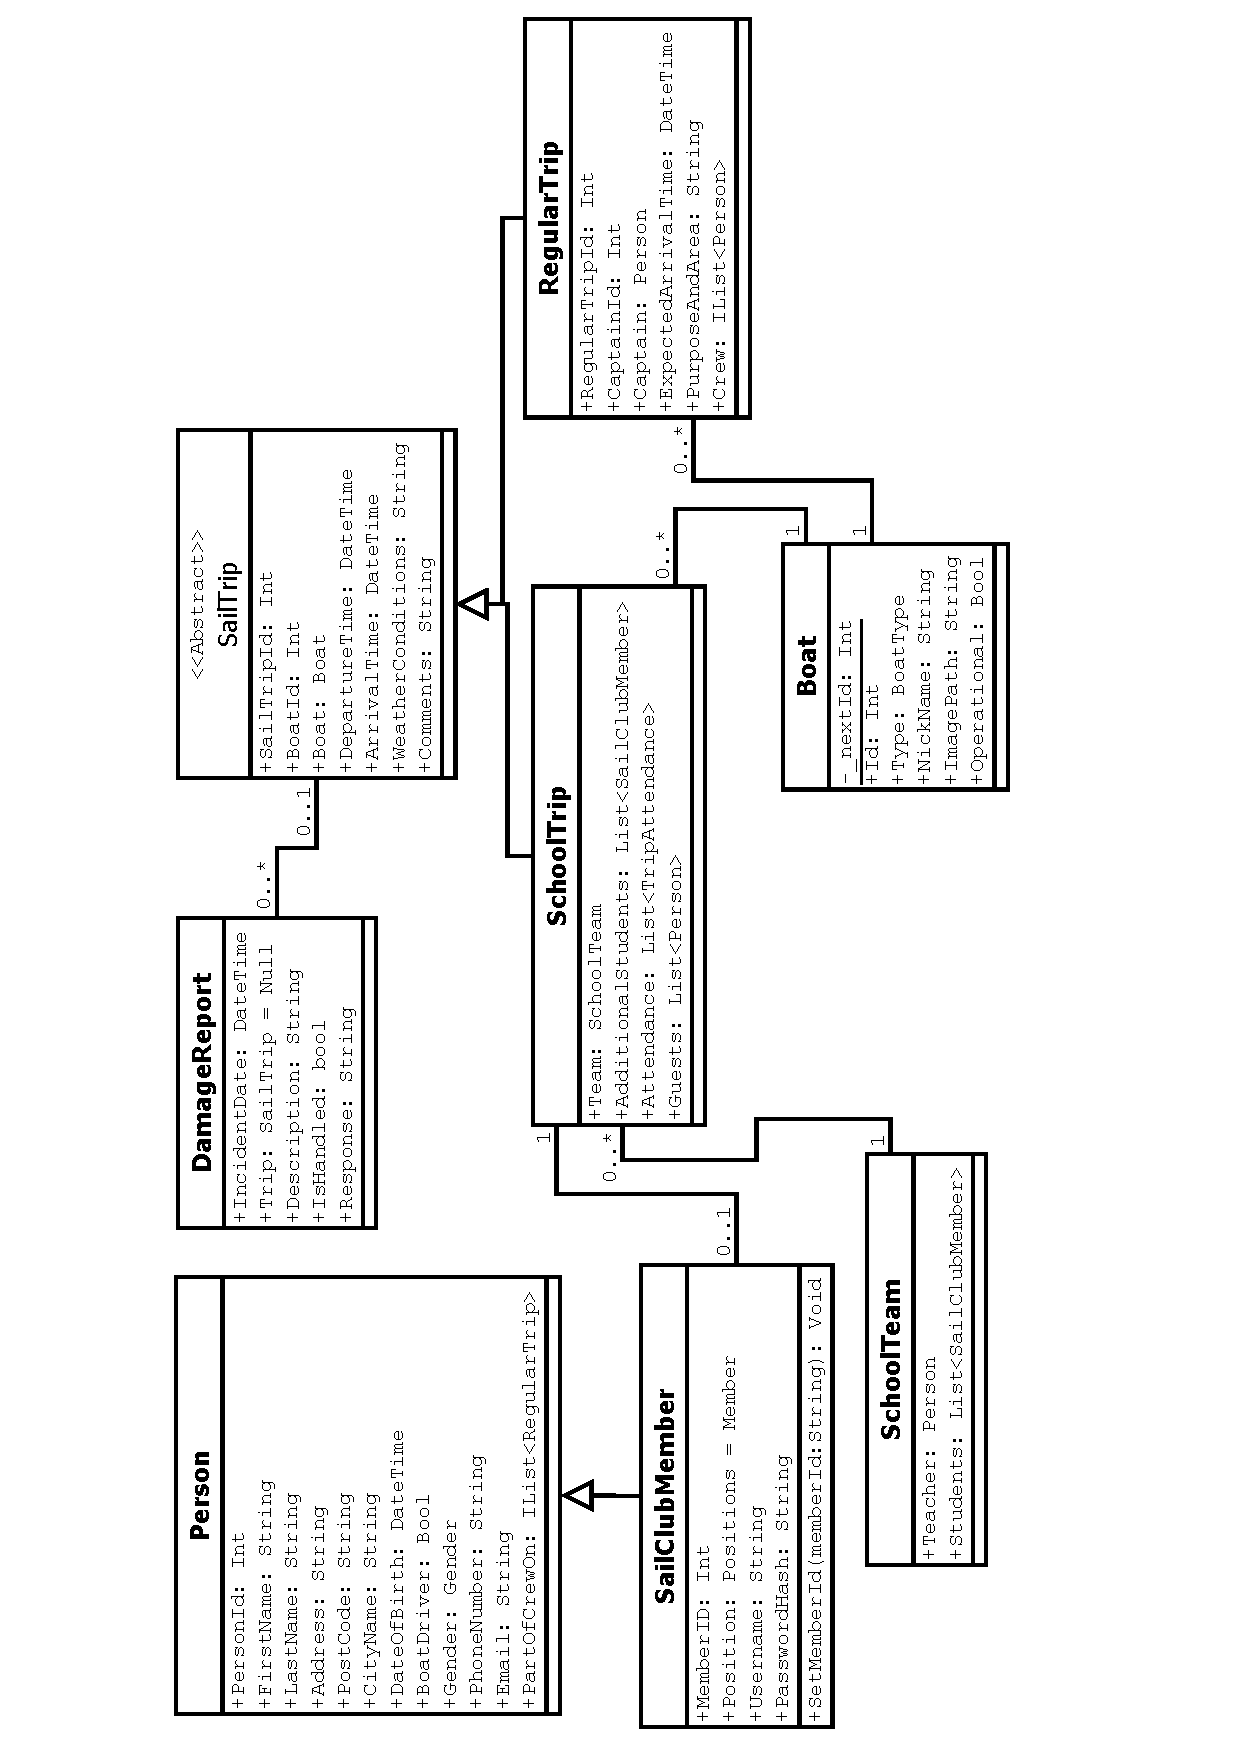
\includegraphics[width=0.70\textwidth]{images/flowcharts/UML.pdf}
  \caption{UML-diagram over klasserne i programmet}
  \label{img:UML}
\end{figure}

\subsection*{Klasse: Person}
\textbf{Formål:}
Formålet med personklassen er at kunne repræsentere personer som vedrører programmet.
Data om disse personer angives som felter i personklassen.

\textbf{Metoder:}
Personklassen har overridet \textbf{ToString()}, som returnerer \textbf{FullName}.

\textbf{Anvendelse:}
Personklassen bruges til at repræsentere alle personer i systemet. 
Gæster repræsenteres direkte som instanser af personklassen. 
Sejlklubbens medlemmer repræsenteres som subklasser af personklassen. 

\subsection*{Klasse: SailClubMember}

\textbf{Formål:}
SailClubMember bruges til at repræsentere medlemmerne i sejlklubben, med undtagelse af de studerende som har en subklasse.

\textbf{Position} feltet angiver hvilken rang, og dermed rettigheder, som et sejlklubmedlem har. 
Dette repræsenteres ud fra en enumeration.

\textbf{Anvendelse:}
SailClubMember bruges til at danne instanser af alle sejlklubbens medlemmer, bortset fra de studerende som er instanser af StudentMember der nedarver fra SailClubMember.

\subsection*{Klasse: StudentMember}
\textbf{Formål:}
Klassen StudentMember indeholder informationer om, hvilke læringsmål eleven har udført i forbindelse med sejlerskolen. 

\textbf{Anvendelse:}
Klassen StudentMember nedarver fra SailClubMember og bruges til at repræsentere eleverne i sejlklubben.

\subsection*{Klasse: Team}

\textbf{Formål:}
Klassen Team har til formål at repræsentere et vilkårligt sejlerskolehold.
Samtidigt inderholder den både en liste over elever og lektioner.

\textbf{Anvendelse:}
Team anvendes til at samle en gruppe elever i sejlerskolen.
Denne samling gør det muligt at håndtere eleverne på holdet på samme tid.

\subsection*{Klasserne: SailTrip og RegularSailTrip}
\textbf{Formål:}
I en tidlig designstruktur var det tænkt at programmet skulle indeholde flere forskellige typer af sejlture, og derfor blev SailTrip-klassen skabt som værende superklasse for sejltursklasser. 
Senere blev ideen om at have flere typer sejlture ændret, og i stedet blev der valgt, at der kun skulle være én sejlturstype. 
SailTrip-klassen er dog bibeholdt i tilfælde af videre udbygning af programmet.
Dog findes der enkelte felter i klasserne, som overlapper hinanden lidt, men felter er også bibeholdt i tilfælde af udbygning til flere typer sejlture.

\textbf{Anvendelse:}
SailTrip-klassen anvendes kun som superklasse for RegularTrip-klassen. 
Hver reservation er en instans af klassen RegularTrip, dette gælder også reservationer for sejlerskolens lektioner.

\subsection*{Klasse: Event}

\textbf{Formål:} 
Denne klasse repræsenterer en begivenhed i sejlklubben.

\textbf{Anvendelse:}
En instans af eventklassen, repræsenterer en begivenhed, der ikke nødvendigvis er sejlrelateret.

\subsection*{Klasse: Logbook}

\textbf{Formål:}
Efter hver sejltur skal der udfyldes en logbog med informationer om sejlturen. 
Denne klasse repræsenterer denne logbog.

\textbf{Anvendelse:}
En instans af klassen Logbook findes på hver sejltur. 
Den udfyldes af personen, som har foretaget reservationen, efter sejladsens fuldførelse. 

\subsection*{Klasse: Lecture}

\textbf{Formål:}
Klassen Lecture indeholder information vedrørende en undervisning. 

\textbf{Anvendelse:}
Denne klasse bruges, når der reserveres en båd til sejlerskolen og samtidigt til at registrere, hvilke læringsmål som blev udført på turen. 

